\documentclass[a4paper, 12pt]{article}

% -- Language --
\usepackage[spanish]{babel}
\usepackage[utf8]{inputenc}

% ----- Fonts -----
% -- Color --
\usepackage{xcolor}
%\definecolor{azul}{RGB}{00,33,99}
\definecolor{azul}{RGB}{35,72,180}

% -- Page Margin --
\usepackage[margin=1in]{geometry}

% -- Espaciados --
\newcommand{\Pspace}{0.5cm}
\newcommand{\Aspace}{0.2cm}

% -- Imagenes --
\usepackage{graphicx}

\title
{
  Probabilidad 2025-1 \\
  Tareas
}

\begin{document}

\maketitle

\begin{center}
    \begin{tabular}{r|l}
        \textbf{Expediente} & \textbf{Nombre} \\ \hline
        219208106 & Bórquez Guerrero Angel Fernando \\
        223203899 & Tostado Cortes Dante Alejandro \\
    \end{tabular}
\end{center}

\rule{\linewidth}{0.3mm}



% ---------- Tarea 1 ----------
\vspace{0.3cm}

\begin{center}
    { \LARGE Tarea 1}
\end{center}

\begin{enumerate}
    % - Problema 1
    \item Si $n(A) = 15$, $n(B) = 20$, y $n(A \cap B) = 10$. Encontrar $n(A \cup B).$ 
    % Respuesta:
    \vspace{\Aspace} \par
        { \color{azul} $n(A \cup B) = n(A) + n(B) - n(A \cap B) = 15 + 20 - 10 = 25$ }


    % - Problema 2
    \vspace{\Pspace}
    \item Una persona tiene 4 camisetas, 5 pantalones, 7 pares de zapatos y 2 sombreros. ¿Cuántos conjuntos diferentes podría vestir?
    % Respuesta:
    \vspace{\Aspace} \par
    { \color{azul} 4 \cdot\ 5 \cdot\ 7 \cdot\ 2 = 280 }


    % - Problema 3
    \vspace{\Pspace}
    \item ¿Cuántos números de tres dígitos se forman utilizando los dígitos 0, 1, 2, 3, 4, 5, 6, 7, 8 y 9? Se permiten dígitos repetidos.
    % Respuesta:
    \vspace{\Aspace} \par
        { \color{azul} $10^{3} = 1000$ } 
\end{enumerate}



% ---------- Tarea 2 ----------
\newpage
\begin{center}
    { \LARGE Tarea 2}
\end{center}

\begin{enumerate}
    %  - Problema 1
    \item Una cerradura de combinación se abrirá cuando se seleccione la opción correcta de tres números (del 1 al 40, contando el 40). ¿Cuántas combinaciones diferentes de la cerradura son posibles?
    % Respuesta:
    \vspace{\Aspace} \par
        { \color{azul} $40^{3} = 64,000$ }


    % - Problema 2
    \vspace{\Pspace}
    \item Cuatro parejas (8 personas) han reservado asientos en una fila para un concierto. ¿En cuántas formas pueden tomar asiento si (a) no hay restricciones para hacerlo? (b) los dos de cada pareja desean sentarse juntos?
    % Respuestas:
    \vspace{\Aspace} \par
    (a) { \color{azul} $8! = 40,320$ }

    \vspace{\Aspace}
    (b) { \color{azul} $4! \cdot 2^{4} = 384$ }
    

    % - Problema 3
    \vspace{\Pspace}
    \item De entre un grupo de 40 personas, ha de seleccionarse un jurado de 12 personas. ¿En cuántas formas puede ser seleccionado el jurado?
    % Respuesta:
    \vspace{\Aspace} \par
        { \color{azul} $_{40}C_{12} = 55,868,534,80$ }

    
    % - Problema 4
    \vspace{\Pspace}
    \item La complejidad de las relaciones interpersonales crece de modo considerable cuando el tamaño del grupo es mayor. Determine el número de relaciones de dos parejas en grupos de (a) 3, (b) 8, (c) 12 y (d) 20 personas.
    % Respuestas:
    \vspace{\Aspace} \par
    (a) { \color{azul} $_{3}C_{2} = 3$ }
    
    \vspace{\Aspace}
    (b) { \color{azul} $_{8}C_{2} = 28$ }
    
    \vspace{\Aspace}
    (c) { \color{azul} $_{12}C_{2} = 66$ }
    
    \vspace{\Aspace}
    (d) { \color{azul} $_{20}C_{2} = 190$ }


    % - Problema 5
    \vspace{\Pspace}
    \item ¿Cuántos arreglos diferentes pueden formarse con una caja de 8 colores, si contiene 4 blancos, 3 azules y 1 rojo?
    % Respuesta:
    \vspace{\Aspace} \par
        { \color{azul} $_{8}C_{4} \cdot\ _{4}C_{3} \cdot\ 1 = 280$ }

    
    \newpage
    % - Problema 6
    \vspace{\Pspace}
    \item Se sacan cinco cartas de un mazo ordinario de 52 cartas de juego. (a) ¿Cuál es la probabilidad de que la mano sacada sea del mismo palo? (b) ¿Cuál es la probabilidad de que la mano sacada sea una escalera? (c) ¿Cuál es la probabilidad de que la mano sacada sea una tercia?
    % Respuestas:
    \vspace{\Aspace} \par
        (a) { \color{azul} $\frac{_{13}C_{5}-10}{_{52}C_{5}} \cdot\ 4 = 0{.}0196$ }
    
    \vspace{\Aspace}
    (b) { \color{azul} $\frac{(4^{5}-4) \cdot\ 10}{_{52}C_{5}} = 0{.}003924$ }
    
    \vspace{\Aspace}
    (c) { \color{azul} $\frac{_{4}C_{3} \cdot\ _{12}C_{2} \cdot\ 4^{2}}{_{52}C_{5}} = 0{.}02113$ }


    % - Problema 7 
    \vspace{\Pspace}
    \item Se sacan cinco cartas de un mazo ordinario de 52 cartas de juego. (a) ¿Cuál es la probabilidad de que la mano sacada sean dos pares? (b) ¿Cuál es la probabilidad de que la mano sacada sea un par? (c) ¿Cuál es la probabilidad de que la mano sacada no tenga ningún juego posible (carta alta)?
     % Respuestas:
    \vspace{\Aspace} \par
    (a) { \color{azul} $\frac{_{13}C_{2} \cdot _{4}C_{2} \cdot _{4}C_{2} \cdot 4(_{11}C_{1})}{_{52}C_{5}} = 0{.}04750 = 47{.}50\%$
    }
    
    \vspace{\Aspace}
    (b) { \color{azul} $\frac{_{13}C_{1} \times\ _{4}C_{2} \times\ 4(_{12}C_{3})}{_{52}C_{5}} = 0{.}02641 = 26{.}41\%$
    }
    
    \vspace{\Aspace}
    (c) { \color{azul}  
        $\frac{_{13}C_{5} \cdot 4^{5}}{_{52}C_{5}} = 0{.}5011 = 50{.}11\%$
    } 
\end{enumerate}



% ---------- Tarea 3 ----------
\newpage
\begin{center}
    { \LARGE Tarea 3}
\end{center}

\begin{enumerate}
    % - Problema 1
    \item En Hermosillo hay 4\% de probabilidades de que el día de independencia se tenga una temperatura baja. ¿Cuál es la probabilidad de que ese día no se tenga una temperatura baja?
    % Respuesta:
    \vspace{\Aspace} \par
    { \color{azul} $100\% - 4\% = 96\%$ }


    % - Problema 2
    \vspace{\Pspace}
    \item En una clase de álgebra y trigonometría hay 18 alumnos de primer año y 15 de segundo. De los 18 de primero, 10 son hombres; de los 15 de segundo, 8 son hombres. Encuentre la probabilidad de que un estudiante elegido al azar sea:
        \begin{table}[h] \hspace{2em}
        \begin{tabular}{c|c c}  % "c|cc" significa: 1ra columna centrada con línea, 2 y 3 centradas
        \hline
        & \textbf{1er año} & \textbf{2do año} \\
        \hline
        \textbf{Hombre} & 10 & 8 \\
        \textbf{Mujer}  & 8 & 7 \\
        \hline
        \textbf{Total}  & 18 & 15 \\
        \hline
        \end{tabular}
    \end{table}
    
    $A$: Son de primer año. (18)
    \newline $B$: Son de segundo año. (15)
    \newline $C$: Es hombre. (18)
    \newline $D$: Es mujer. (15)

    % Respuestas:
    \vspace{\Aspace} \par
    (a) De primero o mujer:
        \\ { \color{azul} $P(A \cup D) = P(A) + P(D) - P(A \cap D) = \frac{18}{33} + \frac{15}{33} - \frac{8}{33} = \frac{25}{33} = 0{.}76 = 76\%$ }

    \vspace{\Aspace}
    (b) De segundo u hombre:
    \\ { \color{azul} $P(B \cup C) = P(B) + P(C) - P(B \cap C) = \frac{18}{33} + \frac{15}{33} - \frac{8}{33} = \frac{25}{33} = 0{.}76 = 76\%$ }


    % - Problema 3
    \vspace{\Pspace}
    \item Determinar la siguiente igualdad $P(A \cup B \cup C) =$
    % Respuesta:
    \vspace{\Aspace} \par
    { \color{azul} $P(A \cup B \cup C) = P(A) + P(B) + P(C) - P(A \cap B) - P(A \cap C) - P(B \cap C) + P(A \cap B \cap C)$ }


    % - Problema 4
    \vspace{\Pspace}
    \item ¿Cuál es la probabilidad de que en un grupo de 60 personas, por lo menos 2 tengan la misma fecha de cumpleaños?
    % Respuesta:
    \vspace{\Aspace} \par
    { \color{azul} 
        $A$: Dos personas cumplen el mismo día.
        \newline $A^{c}$: Nadie cumple el mismo día.
        \newline $P(A^{c}) = \frac{_{365}P_{60}}{365^{60}} = 0{.}0059 = 0{.}59\%$
        \newline $P(A) = 0{.}9941 = 99{.}41\%$
    } 
\end{enumerate}



% ---------- Tarea 4 ----------
\newpage
\begin{center}
    { \LARGE Tarea 4}
\end{center}

\begin{enumerate}
    %  - Problema 1
    \item Juan vive en una gran ciudad y viaja al trabajo diariamente en subterráneo o en taxi. Aborda el subterráneo 80\% del tiempo porque cuesta menos y toma un taxi el otro 20\% del tiempo. Cuando se toma el subterráneo, llega al trabajo a tiempo 70\% de las veces, mientras que llega a tiempo 90\% de las veces cuando viaja en taxi.
    \newline $P(A | B) = \frac{P(A \cap B)}{P(B)} \rightarrow P(B) \times P(A | B) = P(A \cap B)$
    \newline $T$: Viaja en taxi. (20\%)
    \newline $S$: Viaja en subterráneo. (80\%)
    \newline $A$: Llega a tiempo.
    \newline $A | T$: Llega a tiempo dado que tomó un taxi.
    \newline $A | S$: Llega a tiempo dado que tomó el subterráneo.
    % Respuestas:
    \vspace{\Aspace} \par
    (a) ¿Cuál es la probabilidad de que Juan tome el subterrábneo y llegue a tiempo al trabajo en cualquier día dado?
    \\ { \color{azul} 
        $P(A \cap S) = P(S) \cdot P(A | S) = 0{.}8 \cdot 0{.}7 = 0{.}56 = 56\%$
    }

    \vspace{\Aspace}
    (b) ¿Cuál es la probabilidad de que Juan tome un taxi y llegue a tiempo al trabajo en cualquier día dado?
    \\ { \color{azul}  
        $P(A \cap T) = P(T) \cdot P(A | T) = 0{.}2 \cdot 0{.}9 = 0{.}18 = 18\%$    
    }


    % - Problema 2
    \vspace{\Pspace}
    \item Se lanza un dado equilibrado dos veces. Determine si los siguientes pares de eventos son independientes.
    \newline Para que dos eventos sean independientes debe cumplirse que: 
    \newline $P(A \cap B) = P(A) \cdot P(B)$
    % Respuestas:
    \vspace{\Aspace} \par
    (a) A: La suma de los dos resultados es 6. B: El primer resultado es 4.
    \\ { \color{azul} 
        $P(A) = \frac{5}{36}$
        \newline $P(B) = \frac{1}{6}$
        \newline $P(A \cap B) = \frac{1}{36}$
        \newline Dado que $\frac{5}{36} \cdot \frac{1}{6} \neq \frac{1}{36}$ esto nos dice que son eventos dependientes.
    }

    \vspace{\Aspace}
    (b) A: La suma de los dos resultados es 7. B: El segundo resultado es 4.
    \\ { \color{azul} 
        $P(A) = \frac{6}{36} = \frac{1}{6}$
        \newline $P(B) = \frac{1}{6}$
        \newline $P(A \cap B) = \frac{1}{36}$
        \newline Dado que $\frac{1}{6} \cdot \frac{1}{6} = \frac{1}{36}$ esto nos dice que son eventos independientes.
    }
    
    
    \newpage
    % - Problema 3
    \vspace{\Pspace}
    \item Demostrar la siguiente igualdad $P(A | B) = 1 - P(A^{c} | B)$
    \begin{figure}[h]
        \centering
        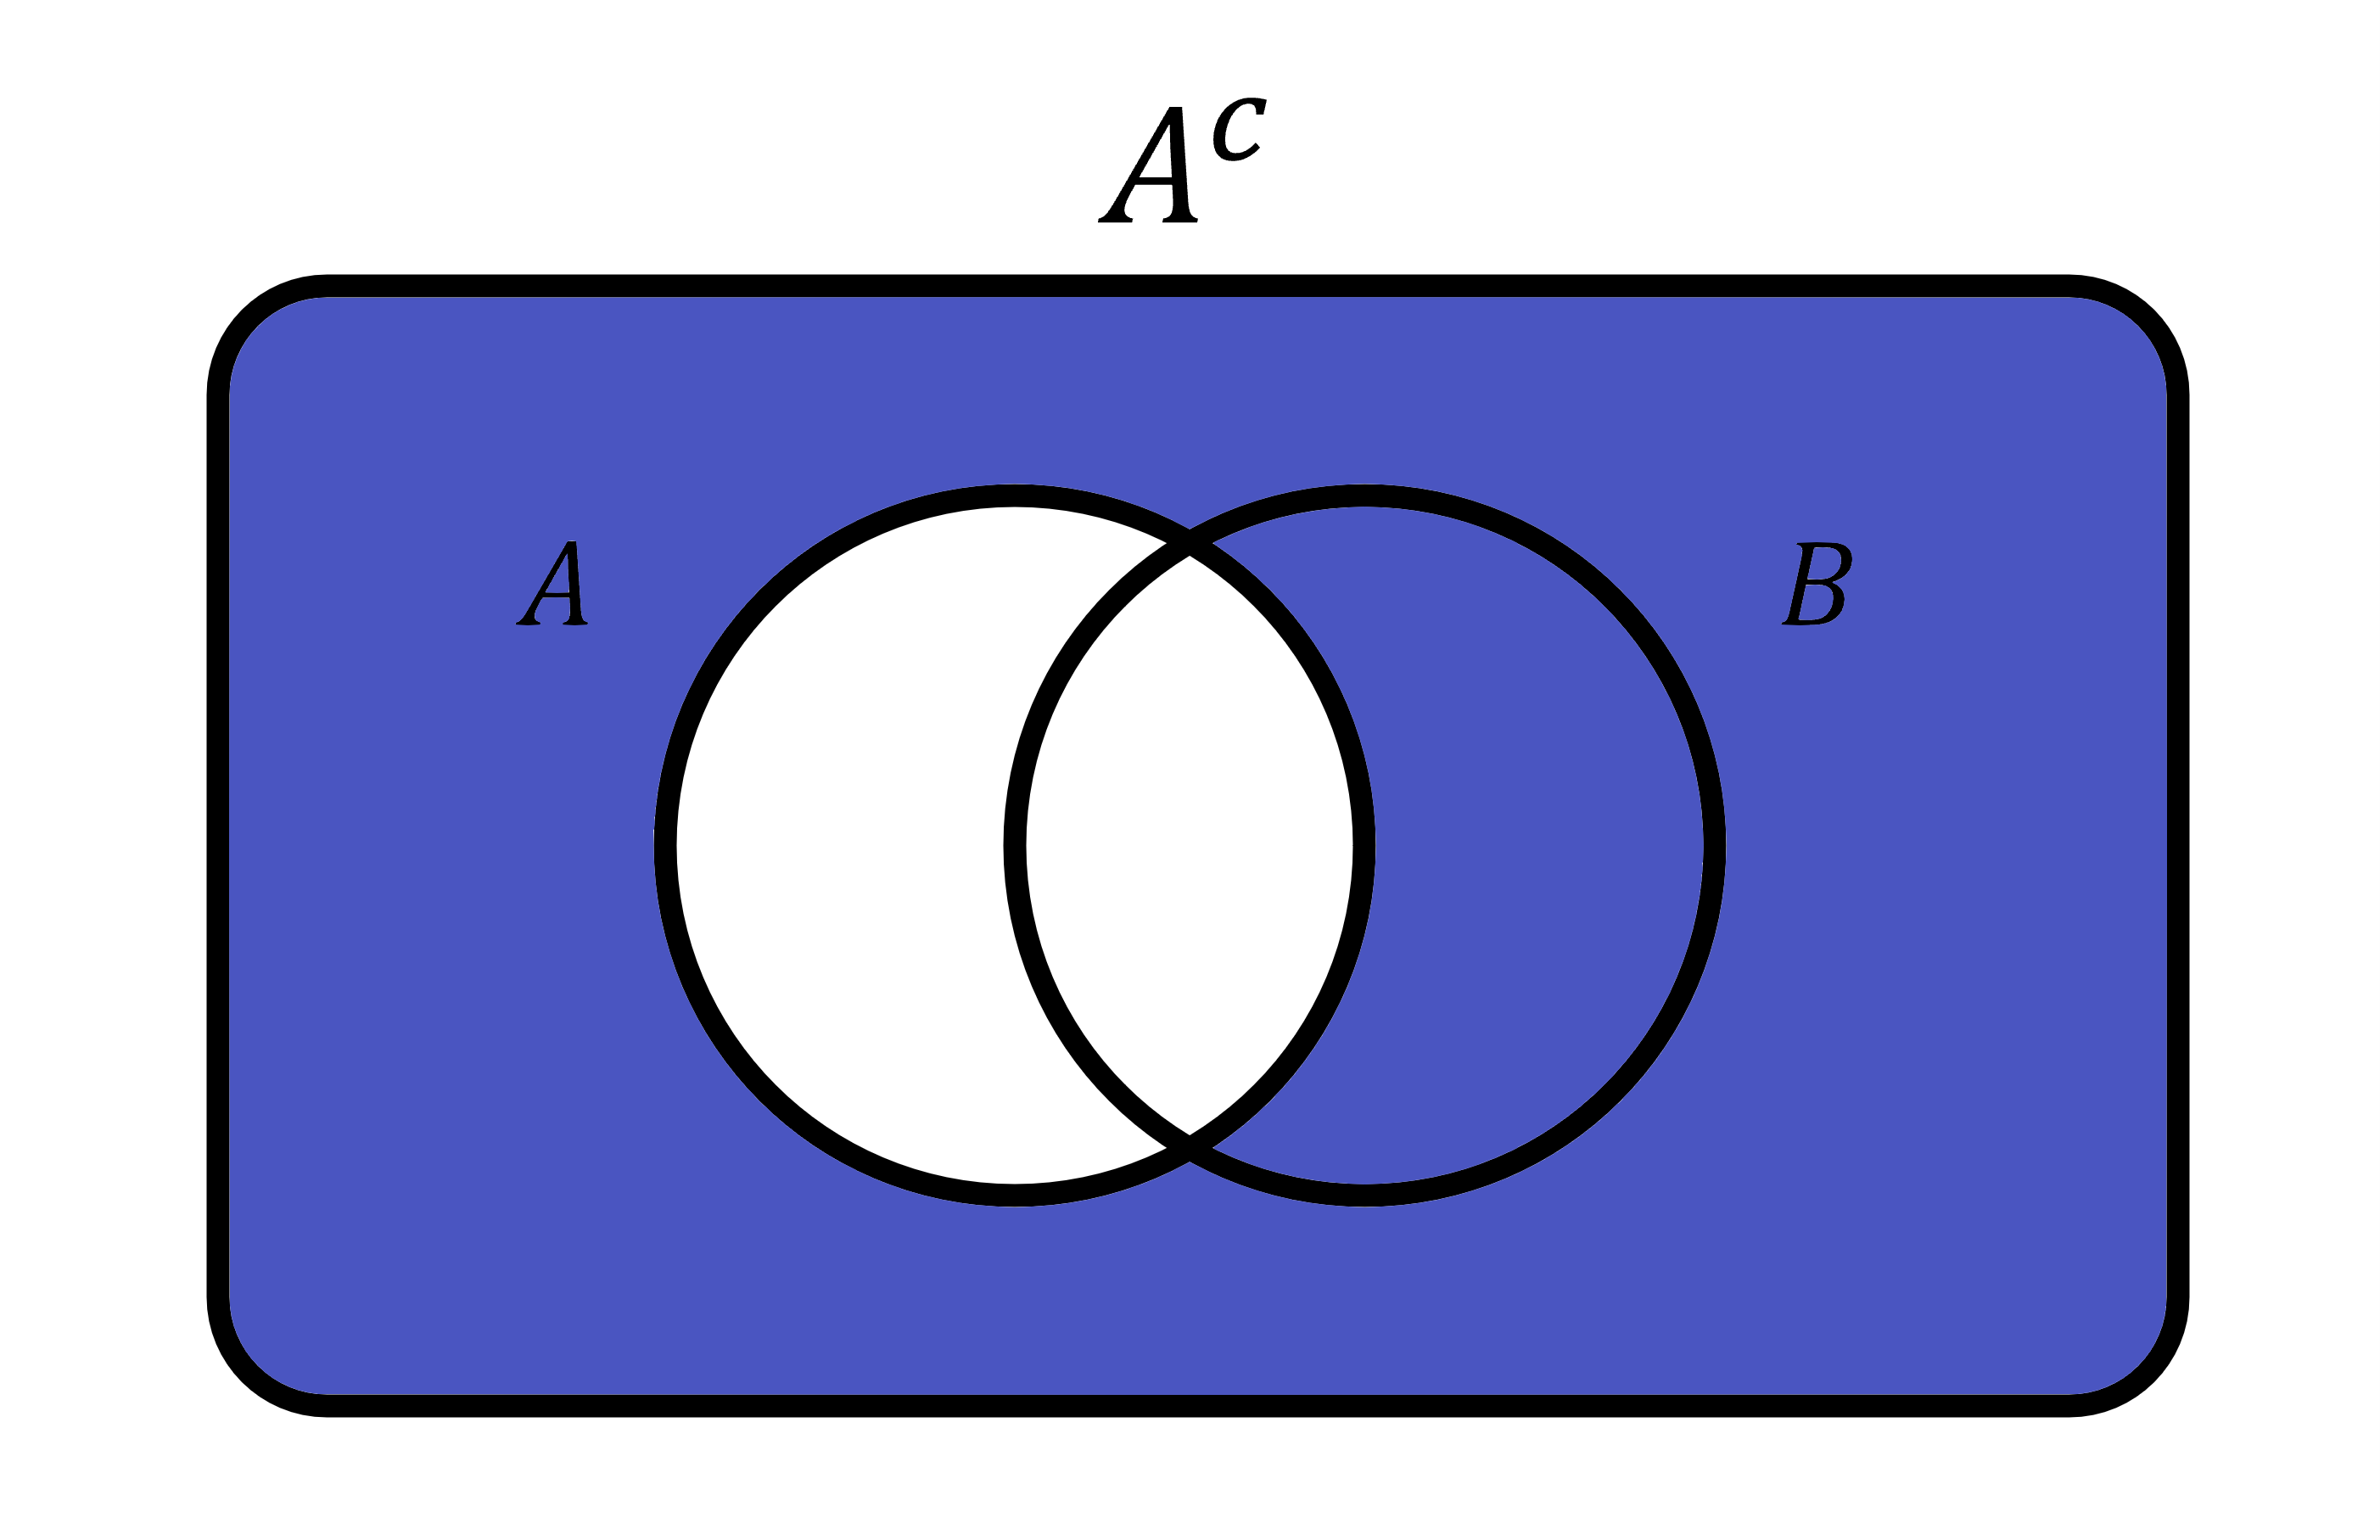
\includegraphics[width=0.4\textwidth]{./Images/Complemento.png}
        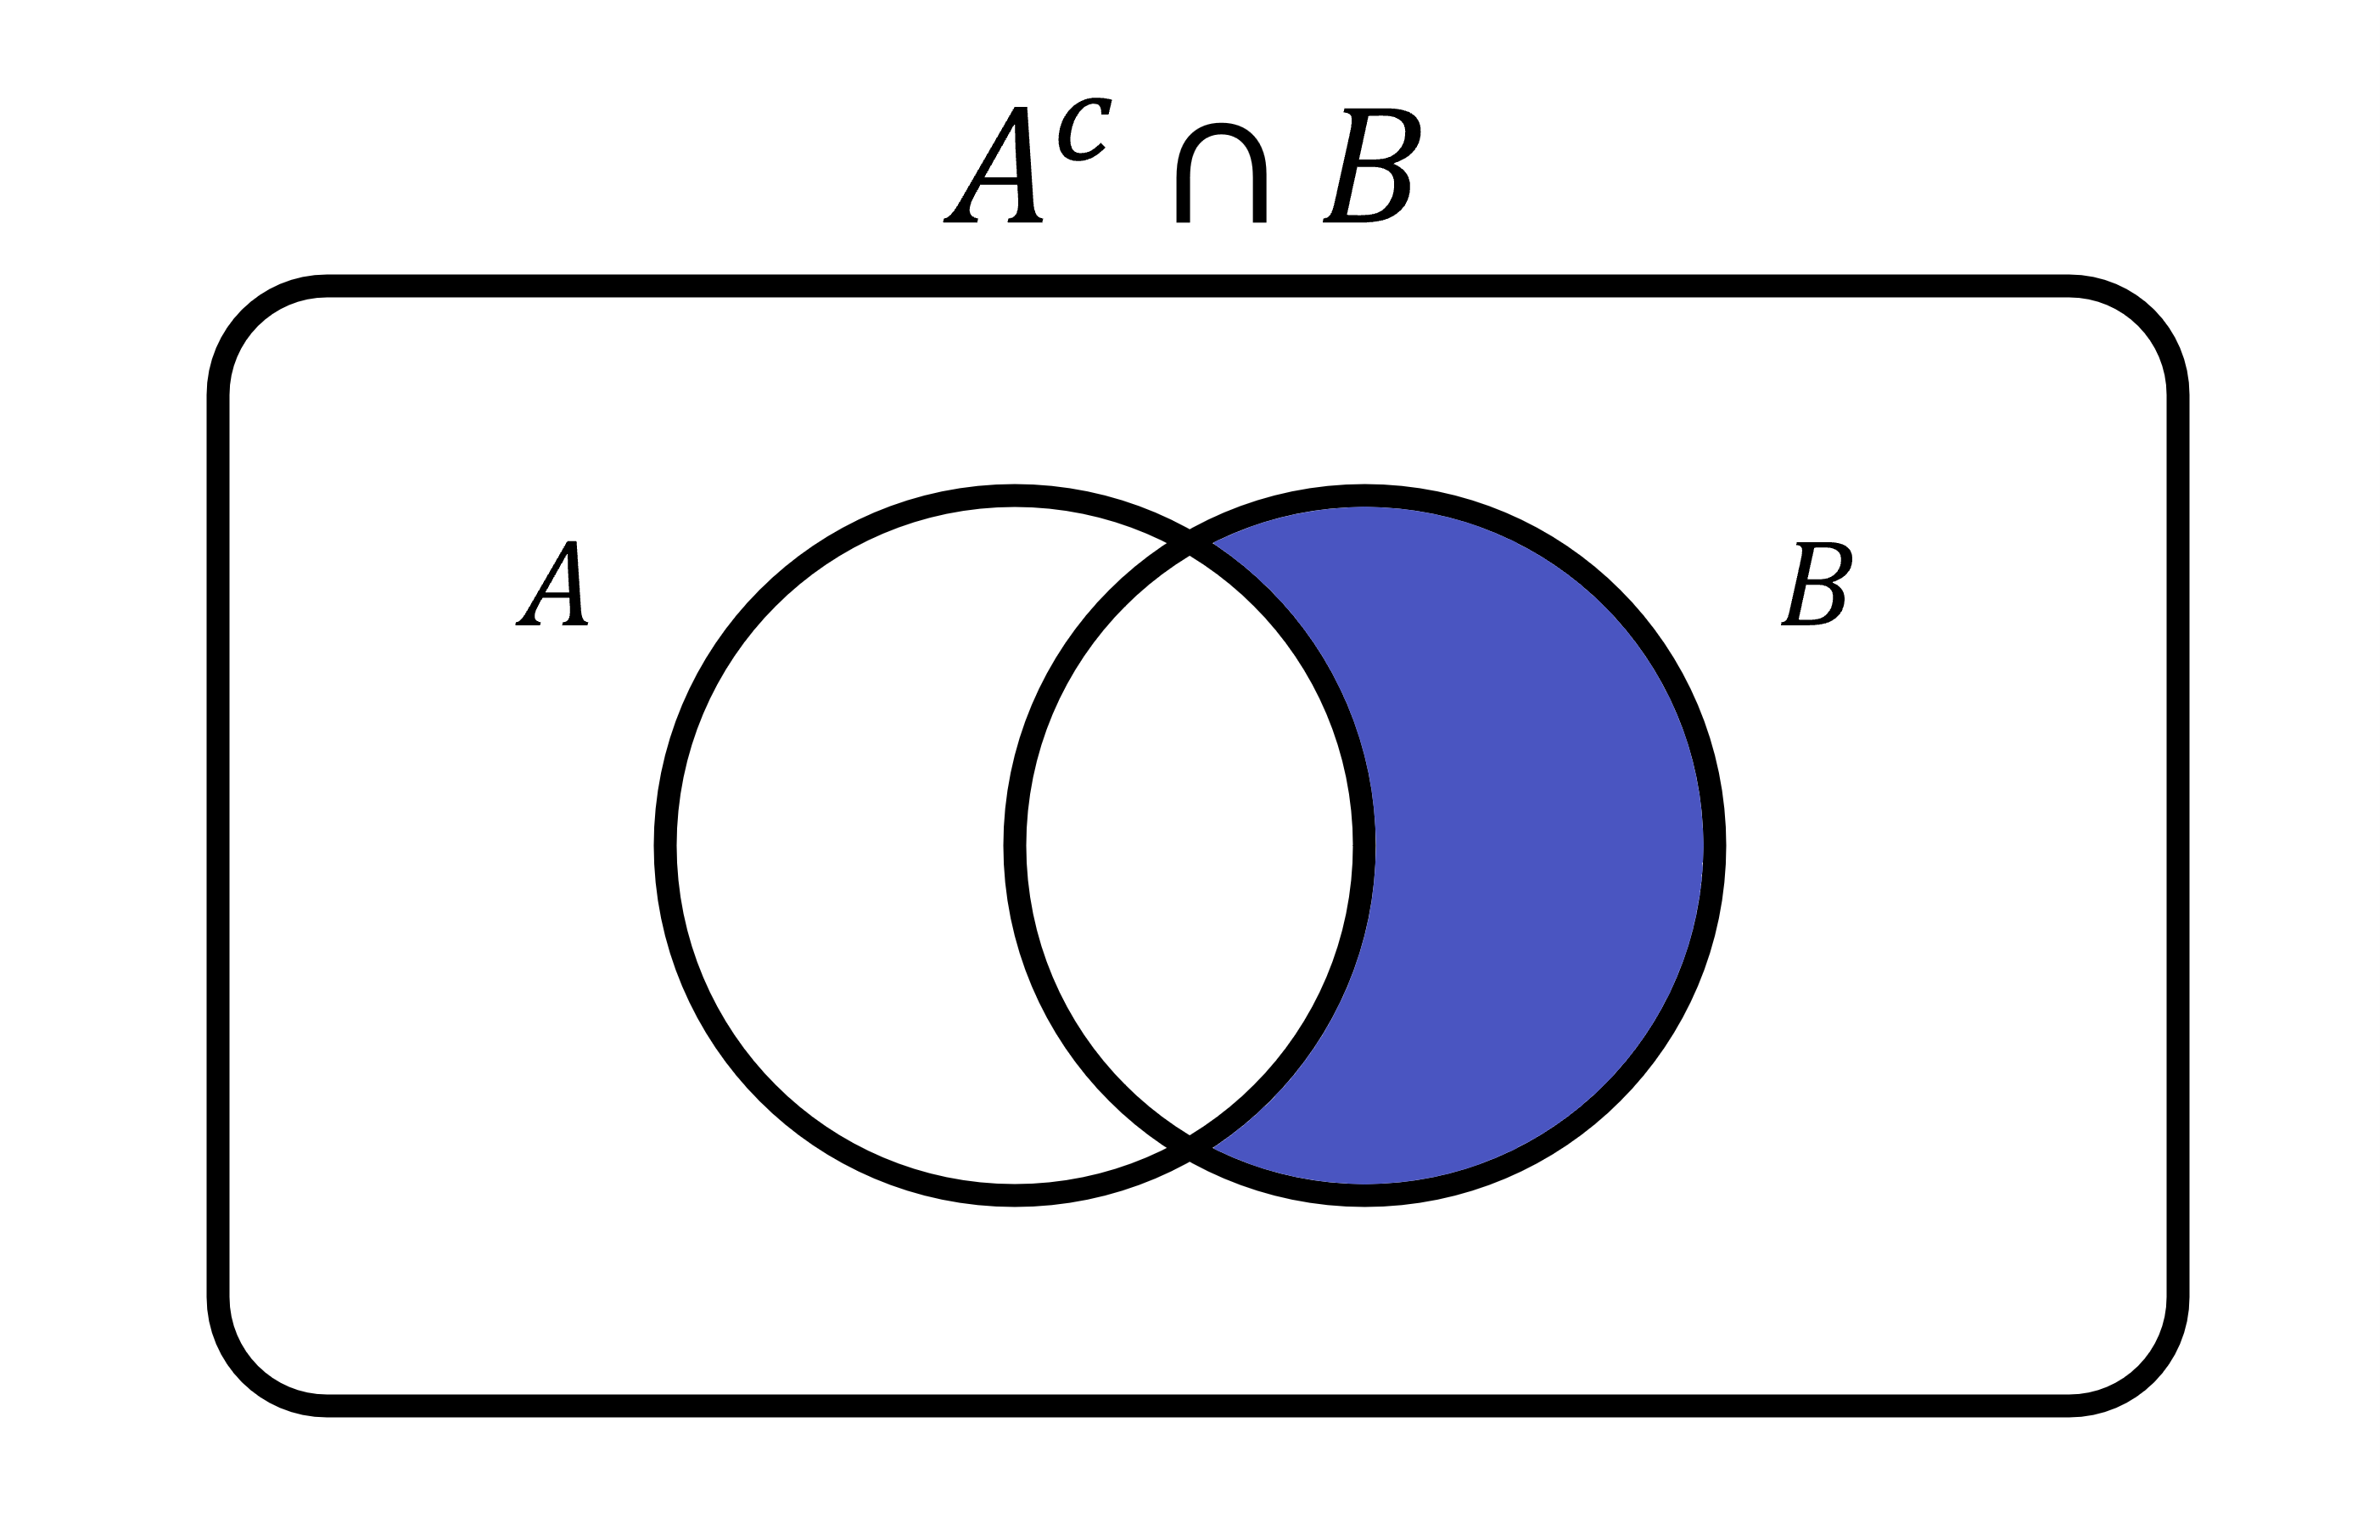
\includegraphics[width=0.4\textwidth]{./Images/Interseccion.png}
    \end{figure}
    % Respuesta:
    \vspace{\Aspace} \par
    { \color{azul} 
        $P(A | B) = 1 - P(A^{c} | B)$
        \newline $\frac{P(A \cap B)}{P(B)} = 1 - \frac{P(A^{c} \cap B)}{P(B)}$
        \newline $P(A \cap B) = P(B) - P(A^{c} \cap B)$
        \newline $P(A \cap B) = P(B) - P(B) + P(A \cap B)$
        \newline $P(A \cap B) = P(A \cap B)$
    }

    
    % - Problema 4
    \vspace{\Pspace}
    \item Si dos eventos son independientes, ¿entonces deben ser disjuntos?
    % Respuesta:
    \vspace{\Aspace} \par
    { \color{azul} 
        Disjuntos: $P(A \cap B) = 0$
        \newline Independientes: $P(A \cap B) = P(A) \cdot P(B)$
        \newline Dos eventos pueden ser independientes y no disjuntos siempre que la probabilidad de ambas sea diferente de 0.
    }


    % - Problema 5
    \vspace{\Pspace}
    \item La paradoja de la caja de Bertrand. Se tienen tres cajas y cada una de ellas tiene dos monedas. La caja A contiene dos monedas de oro. La caja B contiene una moneda de oro y una moneda de plata. La caja C contiene dos monedas de plata. Se selecciona una caja al azar y de allí se escoge una moneda. Si resulta que la moneda escogida es de oro, ¿cuál es la probabilidad de que provenga de la caja con dos monedas de oro?
    \newline $A$: Se escoge la caja A.
    \newline $B$: Se escoge la caja B.
    \newline $C$: Se escoge la caja C.
    \newline $O$: Sale una moneda de oro.
    % Respuesta:
    \vspace{\Aspace} \par
    { \color{azul} 
        $P(A) = P(B) = P(C) = \frac{1}{3}$
        \newline $P(O | A) = 1$
        \newline $P(O | B) = \frac{1}{2}$
        \newline $P(O | C) = 0$
        \newline $P(O) = P(O | A) \cdot P(A) + P(O | B) \cdot P(B) + P(O | C) \cdot P(C) = \frac{1}{2}$
        \newline Teorema de Bayes: $P(A | O) = \frac{P(O | A) \cdot P(A)}{P(O)} = \frac{1 \cdot \frac{1}{3}}{\frac{1}{2}} = \frac{2}{3} = 66{.}67\%$
    }
\end{enumerate}

\end{document}
